\section{Staatsfinanzen}
Formen von Staatseinnahmen:
\begin{enumerate}
	\item Steuern
	\begin{itemize}
		\item Direkte Steuern (auf Einkommen/Gewinn oder Vermögen/Kapital, oft mit Umverteilungskomponenten verbunden)
		\item Indirekte Steuern (auf Markttransaktionen, z.B. MwSt, Energiesteuer, Mikrosteuer auf Finanztransaktionen)
		\item Gebühren (Kostendeckung für spezifische staatliche Leistung)
	\end{itemize}
	\item Verschuldung
	\begin{itemize}
		\item Deckung von Investitionen 
		\item Deckung des laufenden Staatsaufwandes (Staatskonsum)
	\end{itemize}
	\item Inflationssteuer
	\begin{itemize}
		\item "Besteuerung" der Geldhaltung durch Ausweitung der Geldmenge 
	\end{itemize}
\end{enumerate}

\subsection{Steuersystem der Schweiz}
\begin{itemize}
	\item Direkte Steuern (2/3 der Staatseinnahmen) und indirekte Steuern (vor allem MwSt.)
	\item Kantone und Gemeinden (knapp 2/3 der Staatseinnahmen)
	\item Finanzföderalismus (Steuerwettbewerb)
	\item Finanzausgleich (zw. Bund und Kantonen, zw. finanzstarken und -schwachen Kantonen), seit 2004 Neuer Finanzausgleich (NFA)
	\item Progressives Steuersystem, je mehr man verdient desto mehr zahlt man. In der Schweiz zahlt circa 10\% der Bevölkerung rund 50\% der Bundessteuern. 
\end{itemize}	

\subsubsection{Schuldenbremse}
\begin{description}
	\item[Grundsatz] Der Bund hält seine Ausgaben und Einnahmen auf Dauer im Gleichgewicht.
	\item[Ausgabenregel] Der Höchstbetrag der im Voranschlag zu bewilligenden Gesamtausgaben richtet sich unter Berücksichtigung der Wirtschaftslage nach den geschätzten Einnahmen.
	\item[Ausnahme] Bei ausserordentlichem Zahlungsbedarf kann der Höchstbetrag angemessen erhöht werden.
	\item[Sanktionen] Überschreiten die in der Staatsrechnung ausgewiesenen Gesamtausgaben den Höchstbetrag, so sind die Mehrausgaben in den Folgejahren zu kompensieren.
	\item[Umsetzung] Das Gesetz regelt die Einzelheiten.
	\item \textbf{Die Schuldenbremse gibt es auch auf Kantonsebene.}
\end{description}

\begin{multicols}{2}
	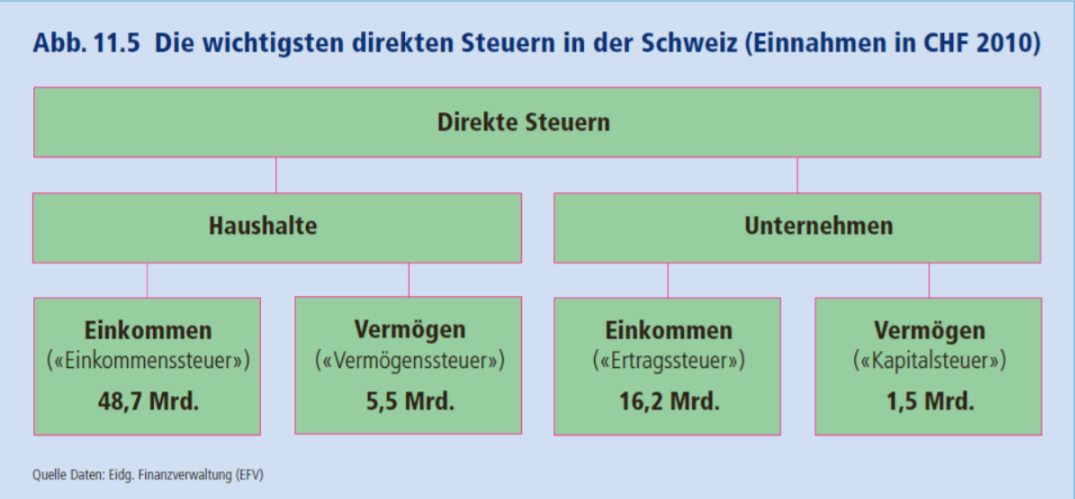
\includegraphics[width=\linewidth]{images/direkteSteuern.png}
	\vfill\null
	\columnbreak
	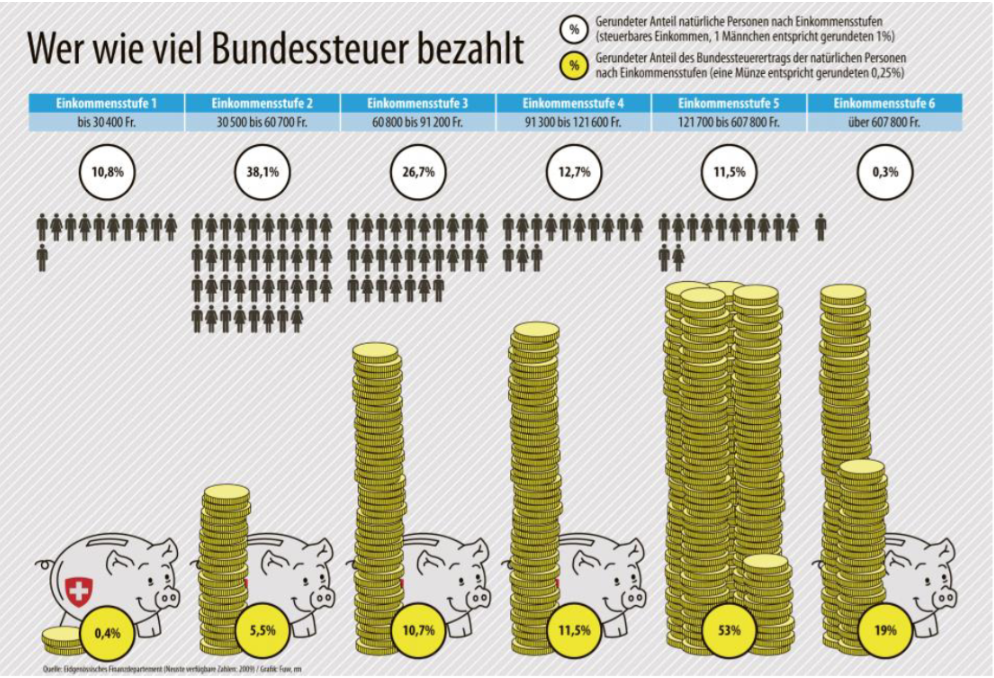
\includegraphics[width=\linewidth]{images/bundessteuern.png}
\end{multicols}

\subsection{Staatsverschuldung}
\begin{itemize}
	\item Verschuldung im Inland führt zum Rückgang inländischer privater Investoren
	\begin{itemize}
		\item Erhöhung der staatlichen Kreditnachfrage auf dem inländischen Kapitalmarkt $\rightarrow$ steigende Kreditzinsen $\rightarrow$ crowding-out der Unternehmensinvestitionen
	\end{itemize}
	\item Verschuldung im Ausland führt zum Rückgang von Exporten
	\begin{itemize}
		\item Erhöhung der staatlichen Kreditnachfrage auf dem ausländischen Kapitalmarkt in ausländischer Währung $\rightarrow$ zwingender Kauf von inländischer Währung für den Erwerb der inländischen Staatsanleihen $\rightarrow$ erhöhte Nachfrage nach inländischer Währung $\rightarrow$ führt zu deren Aufwertung $\rightarrow$ deshalb sinkende Exporte
	\end{itemize}
\end{itemize}
\begin{multicols}{2}
	\subsubsection{Vorteile}
	\begin{description}
		\item[Staatliche Investitionen] Finanzierung von langfristigen Investitionen durch die zukünftigen Generationen (intertemporaler Finanzausgleich)
		\item[Steuerglättung] Jährliche Anpassung der Steuersätze kaum vorstellbar, um jederzeit Budgeteinhaltung zu garantieren
		\item[Makroökonomische Stabilisierung] Ausgleich von konjunkturellen Schwankungen durch Veränderung der staatlichen Nachfrage
	\end{description}
	\vfill\null
	\columnbreak
	\subsubsection{Nachteile}
	\begin{description}
		\item[Verdrängung privater Investitionen] crowding-out von effizienten Investitionen (Effizienz durch Wettbewerb, Konkursrisiko der Unternehmen im Gegensatz zum Staat)
		\item[Verlust des Handlungsspielraums im Budget] Zunehmende Staatsschulden führen zu höheren Zinssätzen für die Verschuldung (Zinslast als zunehmender Budgetposten)
		\item[Verlockung zur Monetarisierung der Verschuldung] Erhebung einer $"$Inflationssteuer$"$
	\end{description}
	\vfill\null
\end{multicols}
\subsubsection{Politisch-ökonomische Gründe für tendenziellen Anstieg der Staatsverschuldung}
\begin{itemize}
	\item Staatsverschuldung ist attraktiver als Steuererhöhung (Sicherung der Wiederwahl)
	\item Stimmentausch Parlament
	\item Trennung von Ausgabenbeschluss und Einnahmenentscheid (keine Sicherung der Finanzierung von Ausgabenbeschlüssen)
	\item Stimmentausch (gegenseitige Unterstützung der Parlamentarier, um Vorteile für die eigene Interessengruppe sicherzustellen)
\end{itemize}

\subsubsection{Europäischer Vergleich}
\begin{multicols}{2}
	\begin{description}
		\item[Inflationssteuer] Einnahmen des Staates durch übermässige Geldschöpfung
		\item[Explizite Staatsschuld] Schulden durch Kredite
		\item[Implizite Staatsschuld] alle zukünftigen Versprechen (Renten, Versicherung etc.)
	\end{description}
	\vfill\null
	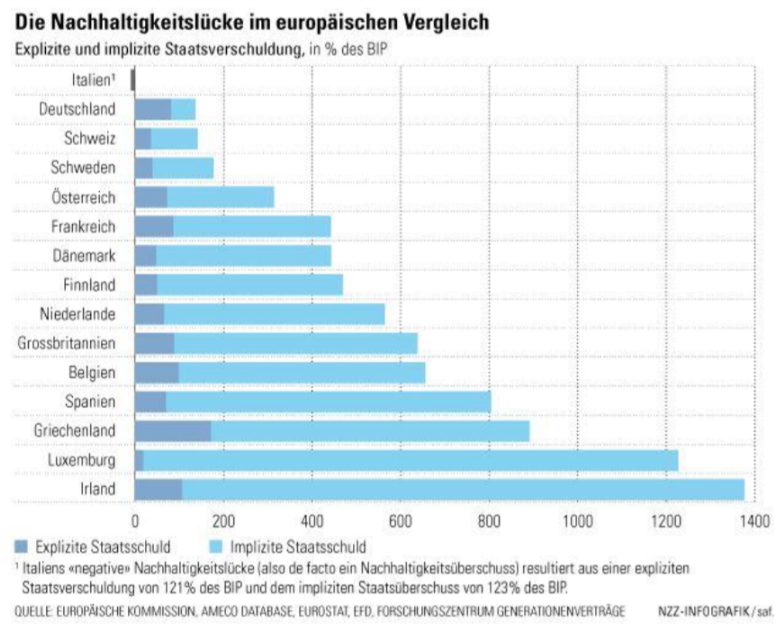
\includegraphics[width=\linewidth]{images/nachhaltigkeitsluecke.png}	
\end{multicols}
	
\subsubsection{Zukunftsschulden der Schweiz}
\begin{multicols}{2}
	Die jungen Generationen werden im Vergleich zu den heutigen Rentnern gemäss den Studienautoren erheblich stärker belastet. Sollte die AHV-Finanzierungslücke bspw. durch eine Erhöhung der MwSt. ab 2025 geschlossen werden, würde sich die Mehrbelastung für eine im Jahr 2010 geborene Person auf 1590Fr. pro Lebensjahr gegenüber einer Person des Jahrgangs 1949 belaufen.\\
	Die Studie stellt ausserdem einen Zusammenhang zwischen der Altersvorsorge und den öffentlichen Haushalten her. Die \textbf{implizite Staatsverschuldung} der Schweiz liegt demnach bei 167.4\% des BIP. Hinzu kämen noch die \textbf{expliziten Staatsschulden} von 35.5\% des BIP (im Jahr 2011).
	\vfill\null
	\columnbreak
	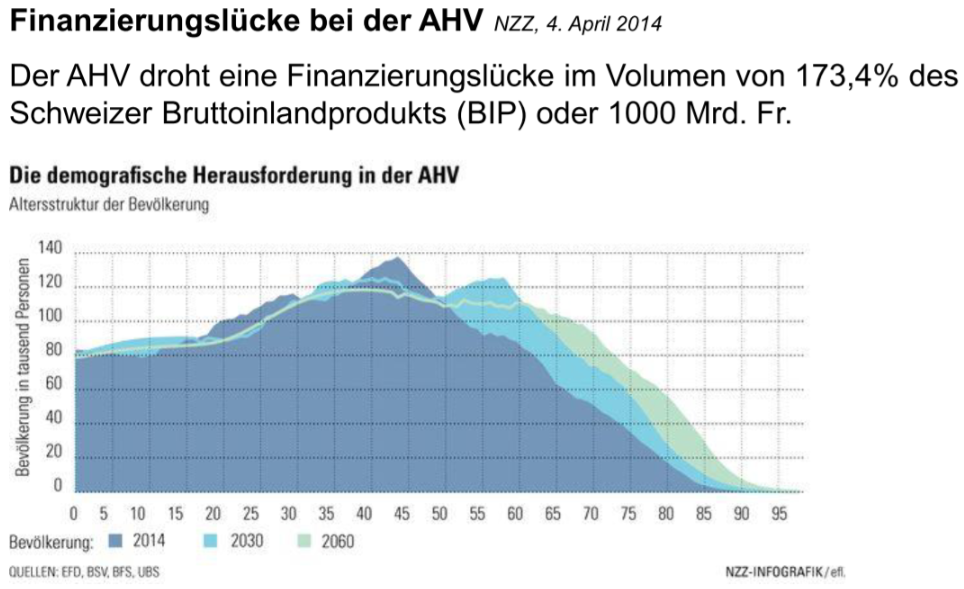
\includegraphics[width=\linewidth]{images/zukunftsschulden.png}
\end{multicols}
